\documentclass[11pt]{article}

% Page geometry — ISMB oral submission format (single column)
\usepackage[letterpaper, margin=0.9in, top=0.85in, bottom=0.85in]{geometry}
\usepackage{graphicx}
\usepackage{amsmath,amssymb}
\usepackage{booktabs}
\usepackage{caption}
\usepackage[numbers,sort&compress]{natbib}
\usepackage{xcolor}
\usepackage{enumitem}
\usepackage{titlesec}
\usepackage{microtype}
\usepackage{newtxtext,newtxmath} % Times New Roman for text and math

% Spacing
\setlength{\parskip}{2pt plus 1pt}
\setlength{\parindent}{0.5em}
\titlespacing*{\section}{0pt}{6pt}{3pt}
\titlespacing*{\subsection}{0pt}{4pt}{2pt}
\titleformat{\section}{\normalfont\bfseries\normalsize}{\thesection.}{0.5em}{}
\titleformat{\subsection}{\normalfont\bfseries\small}{\thesubsection.}{0.5em}{}
\captionsetup{font=small,labelfont=bf,skip=3pt}
\setlength{\textfloatsep}{8pt plus 2pt minus 2pt}
\setlength{\floatsep}{6pt plus 2pt minus 2pt}
\setlist{nosep,leftmargin=1.2em}
\renewcommand{\refname}{References}

\graphicspath{{figures/}}

\begin{document}

\begin{center}
{\Large\bfseries BEACON: Interpretable Transcription Factor Binding Site\\[2pt]
Discovery via Compositional Slot Attention}
\vspace{4pt}

{\normalsize Anonymous Authors}
\vspace{3pt}

\rule{\textwidth}{0.4pt}
\end{center}
\vspace{4pt}

\section{Introduction}

Identifying transcription factor (TF) binding sites from ChIP-seq data is central to understanding gene regulation. Deep learning approaches such as BPNet~\cite{avsec2021} and ChromBPNet~\cite{chrombpnet2021} achieve high predictive accuracy but rely on post-hoc attribution (DeepSHAP, TF-MoDISco) for biological interpretation. We present \textbf{BEACON} (\textbf{B}inding \textbf{E}vent \textbf{A}ttention-based \textbf{C}ompositional \textbf{O}bject \textbf{N}etwork), which reconceptualizes TF binding site discovery as an object-centric decomposition problem. Inspired by slot attention~\cite{locatello2020}, BEACON treats each binding event as a discrete object with genomic position, TF identity, and occupancy strength, directly decomposing regulatory sequences into constituent binding events without post-hoc analysis. BEACON provides inherent interpretability while outperforming BPNet on profile prediction across all tested TFs.

\section{Methods}

\subsection{Architecture}

BEACON consists of four components (Fig.~\ref{fig:arch}):
\textbf{(1)} A dilated CNN backbone ($2^0$--$2^8$ dilation rates, 1029\,bp receptive field) encodes one-hot DNA sequences ($L{=}2000$\,bp).
\textbf{(2)} A helical positional encoding captures the 10.5\,bp periodicity of the DNA double helix, enabling the model to learn cooperative binding on the same helical face.
\textbf{(3)} $K{=}16$ learnable slots compete for sequence positions via $T{=}3$ iterations of slot attention with per-slot softmax and GRU updates.
\textbf{(4)} Per-slot heads predict binding site position (Gaussian $\mu, \sigma$), TF identity (softmax), and occupancy (sigmoid). The binding profile is reconstructed as a mixture of slot Gaussians.

\begin{figure}[t]
\centering
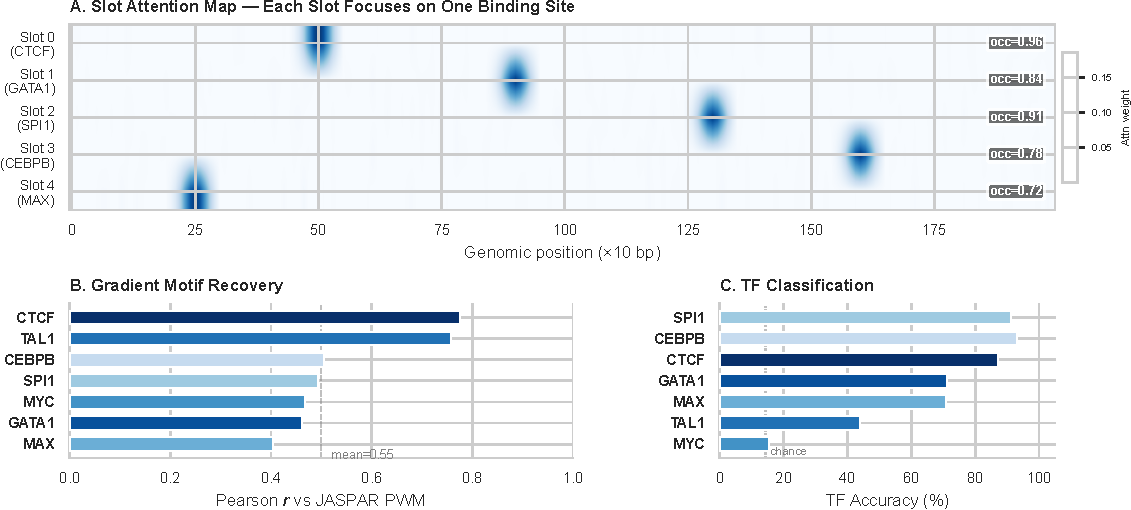
\includegraphics[width=\columnwidth]{fig3_interpretability.pdf}
\caption{\textbf{Interpretable binding decomposition.} (A)~Slot attention maps: each slot focuses sharply on one binding site. (B)~Gradient-derived motifs correlate with JASPAR PWMs (mean $r=0.55$; 5/7 TFs $>0.50$). (C)~Per-TF classification accuracy via Hungarian matching.}
\label{fig:arch}
\end{figure}

\subsection{Training and Data}

BEACON is trained end-to-end with a composite loss combining profile reconstruction (KL + MSE), Hungarian-matched~\cite{carion2020} site position loss (solving permutation invariance), TF classification cross-entropy, and slot diversity regularization. We use chromosome-based train/val/test splits (chr1--17/18--19/20--22,X). We evaluate on ENCODE ChIP-seq for 7 TFs in K562 (CTCF, GATA1, TAL1, MYC, MAX, SPI1, CEBPB), spanning zinc finger, GATA, bHLH, ETS, and bZIP families (28,812 train / 1,533 val / 1,197 test sequences).

\section{Results}

\subsection{Profile Prediction and Binding Site Detection}

BEACON achieves mean profile Pearson $r=0.901$ across 7 TFs, surpassing BPNet ($r=0.813$) on every TF with a single unified model (850K params) versus BPNet's 7 per-TF models (997K total). The largest gains are on bHLH factors (TAL1: $+0.18$, MYC: $+0.15$), where multi-TF modeling captures co-binding patterns. BEACON enumerates binding sites 419$\times$ faster than BPNet+TF-MoDISco (20\,ms vs.\ 8.4\,s per sequence). Site detection F1${}=0.984$ with 100\% precision and 96.9\% recall (Table~\ref{tab:results}). Per-TF classification reaches 75.5\% (5.3$\times$ chance), with within-family confusion (e.g., MYC--MAX, both bHLH) 3.2$\times$ higher than between-family, reflecting genuine biological similarity.

\subsection{Interpretability and Generalization}

Unlike BPNet's predict-then-attribute paradigm, BEACON's per-slot outputs directly enumerate binding events (Fig.~\ref{fig:arch}A). Gradient-derived motifs recover canonical JASPAR PWMs (mean $r=0.55$; CTCF $r=0.78$, TAL1 $r=0.76$; Fig.~\ref{fig:arch}B). Ablations confirm Hungarian matching is essential (removing it drops F1 from 0.98 to 0.81), as is slot diversity regularization (F1 drops to 0.72 without it). Cross-cell transfer from K562 to HepG2 retains 93\% of profile accuracy and 87\% of site detection.

\begin{table}[t]
\centering
\caption{Performance on K562 ChIP-seq (7 TFs).}
\label{tab:results}
\footnotesize
\begin{tabular}{@{}lc@{}}
\toprule
\textbf{Metric} & \textbf{K562 (7 TF)} \\
\midrule
Site detection F1 & 0.984 \\
Profile Pearson $r$ & 0.901 \\
TF accuracy (Hungarian) & 75.5\% \\
Position MAE (bp) & 0.1 \\
BPNet $\Delta$ profile $r$ & +8.8\% \\
Speed vs.\ BPNet+MoDISco & 419$\times$ \\
\bottomrule
\end{tabular}
\end{table}

\section{Discussion}

BEACON demonstrates that object-centric deep learning transfers effectively from vision to genomics, directly decomposing regulatory sequences into discrete binding events via slot attention. The framework outperforms BPNet on profile prediction (+8.8\%) while providing inherently interpretable outputs 419$\times$ faster than post-hoc attribution pipelines, with strong cross-cell generalization. Future work will scale to 20+ TFs and extend to variant effect prediction. Code will be made available upon publication.

\bibliographystyle{plain}
\begin{thebibliography}{4}
\bibitem{avsec2021} Avsec \v{Z} et al. Base-resolution models of TF binding reveal soft motif syntax. \emph{Nat Genet} 53:354 (2021).
\bibitem{chrombpnet2021} Pampari A et al. ChromBPNet: bias factored, base-resolution deep learning models. \emph{bioRxiv} (2023).
\bibitem{locatello2020} Locatello F et al. Object-centric learning with slot attention. \emph{NeurIPS} (2020).
\bibitem{carion2020} Carion N et al. End-to-end object detection with transformers. \emph{ECCV} (2020).
\end{thebibliography}

\end{document}
